\chapter{Storia del filtraggio e principali problemi affrontati}
Le immagini hanno un ruolo fondamentale nelle nostre vite, viviamo di immagini, ne guardiamo tutti i giorni in tutti i contesti, la percezione visiva è sempre il nostro primo riferimento senza la quale ci si sentiamo persi.\\
Viviamo in una società consapevole di ciò e che sfrutta questo aspetto quanto più possibile nei campi più disparati, fotografie, radiografie, ecografie, poster pubblicitari, progetti, etc.\\
E' quindi un problema sempre di grande interesse cercare di sfruttarle al meglio, a tal fine esistono metodi cosìdetti di "filtraggio", tramite i quali intendiamo migliorare la qualità delle nostre immagini, mettere in risalto determinate caratteristiche o nasconderne altre.
\section{Storia del filtraggio}
Anche prima dell'avvento dei computer esisteva l'elaborazione delle immagini. Esisteva infatti dei procedimenti, detti “mascherature”, che servivano a ridurre o esaltare le differenze di luce nella foto.\\La mascheratura avveniva durante la fase di stampa su carta, ossia quando il negativo pellicola veniva proiettato sulla carta fotografica mediante l’ingranditore.

\vspace{1em}\noindent 
Qui, lo “stampatore” usava una serie di metodi per far si che su certe zone della carta andasse più o meno luce di quella che sarebbe arrivata passando attraverso il negativo.

Ad esempio la tecnica nota come "altissimo contrasto" permetteva di avere foto con soli bianchi e soli neri, il viraggio invece serviva a dare un tono di colore alla foto, che restava comunque un bianco e nero: famoso il viraggio tono seppia.

\vspace{1em} \noindent
Le prime applicazioni delle immagini digitali sono state sui giornali negli anni 20. Non esistevano veri e propri computer, il segnale era trasmesso tramite telegrafo simulando dei mezzitoni.
In particolare, il sistema di trasmissione di immagini via cavo Bartlane era una tecnica inventata nel 1920 per trasmettere immagini di giornali digitalizzate su linee sottomarine tra Londra e New York.

\noindent Il sistema di trasmissione di immagini via cavo Bartlane generava sia sul trasmettitore che sul ricevitore una scheda dati perforata o un nastro che veniva ricreato come immagine.

\begin{figure}[htb] \centering
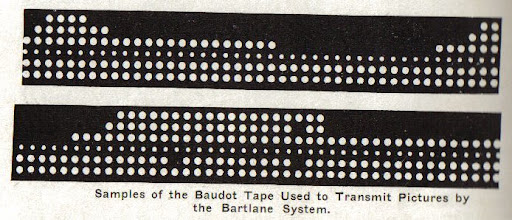
\includegraphics[scale=0.7, trim = 0 1.1cm 0 0, clip]{Pictures/nastro Bartlane.jpg}
\caption{Nastro dati codificante un'immagine.}\label{fig:figura}
\end{figure}

\noindent
In questo modo riusciva a codificare immagini in bianco e nero in cinque diverse gradazioni di grigio, capacità poi ampliata a 15 gradazioni nel 1929.

\begin{figure}[htb] \centering
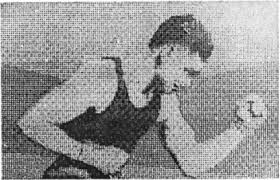
\includegraphics[scale=0.5, trim = 0 1.1cm 0 0, clip]{Pictures/img del 1921 a 5 gradazioni di grigio.jpg}
\qquad\qquad
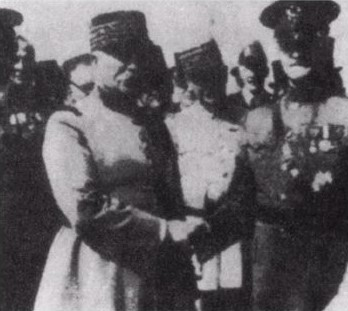
\includegraphics[scale=1.7, trim = 0 1.1cm 0 0, clip]{Pictures/img del 1929 a 15 gradazioni di grigio.jpg}
\caption{La prima immagine risale al 1921 ed è composta da 5 gradazioni di grigio.\\ 
La seconda è del 1929 ed è composta da 15 gradazioni di grigio.}\label{fig:figura}
\end{figure}
\vspace{1em} \noindent
Questa è la nascita delle immagini digitali, anche se non sono trattate da computer e quindi codificate in maniera differente. Inoltre in questa fase non abbiamo una vera e propria elaborazione delle immagini, ma solo una trasmissione e la successiva stampa.

\vspace{1em} \noindent
Nel 1957, Russell A. Kirsch produsse un dispositivo che generava dati digitali che potevano essere archiviati in un computer; questo utilizzava uno scanner a tamburo e un tubo fotomoltiplicatore.\\
Negli anni immediatamente successivi questo porto a notevoli sviluppi.

\vspace{1em} \noindent
Nel 1960 presso il Jet Propulsion Laboratory, il Massachusetts Institute of Technology, i Bell Laboratories, l'Università del Maryland, e altre strutture di ricerca svilupparono molte delle tecniche di elaborazione digitale di immagini (o della trasformazione di immagini digitali come spesso veniva chiamata) al fine di evitare le debolezze operative delle fotocamere a pellicola per missioni scientifiche e militari.\\
Queste trovarono poi applicazione in immagini satellitari, immagini medicali, videocitofono, riconoscimento ottico dei caratteri, e miglioramenti fotografici.

Il costo dell'elaborazione in quel periodo era piuttosto alto con l'apparecchiatura di elaborazione. Le cose cambiarono negli anni settanta, quando computer più economici e hardware dedicato furono resi disponibili sul mercato.\\
Le immagini allora potevano essere elaborate in tempo reale, l'elaborazione digitale sostituisce così i vecchi metodi a pellicola per molti scopi.

\vspace{1em} \noindent
Negli anni 2000, grazie all'avvento di computer più veloci, l'elaborazione delle immagini digitali diventò la forma più comune di elaborazione delle immagini e, in generale, divenne il metodo più utilizzato data la sua versatilità e il basso costo.

La tecnologia di elaborazione delle immagini digitali per applicazioni mediche è stata inserita nel 1994 nella Hall of Fame della Space Foundation.


\section{Principali problemi di elaborazione digitale}

Al giorno d'oggi i nostri computer ci permettono una vasta gamma di elaborazioni digitali, ce ne sono alcuni, più semplici ma di notevole interesse, ormai già perfezionati ed altri che sono ancora oggetto di studio.

\subsection{Rotazioni, riflessioni,etc}
Le più semplici in assoluto riguardano "movimenti rigidi" come la traslazione o la rotazione, o anche omeomorfismi come la riflessione. Questi sono molto utili per introdurre i primi concetti matematici, come l'impiego di matrici.\\
Definiamo una matrice di trasformazione che moltiplicata per un vettore di coordinate ci rstituisca un altro vettore di coordinate. Questo vuol dire che quel punto va spostato dalle coordinate in cui si trovava a quelle appena calcolate. Ad esempio  

$$
{\begin{bmatrix}
-1&0&0\\
0&1&0\\
0&0&1
\end{bmatrix}}
$$

\noindent
E' una matrice di riflessione lungo l'asse verticale, infatti: 

$$
{\begin{bmatrix}
-1&0&0\\
0&1&0\\
0&0&1
\end{bmatrix}}
\begin{bmatrix}
x\\y\\1
\end{bmatrix}
=
\begin{bmatrix}
-x&y&1
\end{bmatrix}
$$	

\vspace{1em} \noindent
Cioè ogni punto rimane alla stessa ma cambia la propria x con -x, che è esattamente ciò che intendiamo per riflessione lungo l'asse verticale.

\newpage \noindent 
Altri esempi possono essere:

\begin{align*}
&\begin{bmatrix}
1&0&0\\
0&-1&0\\
0&0&1
\end{bmatrix}&-&
\text{Riflessione lungo l'asse orizzontale}\\
\\
&\begin{bmatrix}
2&0&0\\
0&1.5&0\\
0&0&1
\end{bmatrix}&-&
\text{Scalamento}\\
\\
&\begin{bmatrix}
\cos(\theta )&\sin(\theta )&0\\
-\sin(\theta )&\cos(\theta )&0\\
0&0&1
\end{bmatrix}&-&
\text{Rotazione di un angolo theta}\\
\end{align*}



\subsection{Cambio prospettiva}
Una delle trasformazioni più semplici è quella del cambio prospettiva. Una volta compresa la questa trasformazione si è fatto anche un primo passo per parlare di warping, di cui parleremo più avanti.

\vspace{1em} \noindent
Supponiamo di avere la foto di un documento e di volerla migliorare in modo da estrarne solo il documento e che i suoi bordi concidano quindi con i bordi dell'immagine.

\vspace{1em} \noindent
In genere la cosa più semplice ed affidabile è quella di far scegliere i 4 angoli del documento ad un utente. Volendo automatizzare il processo possiamo però scegliere un'altra strada, ossia estrarre i bordi dell'immagine e cercare tra questi quelli che formano un trapezio, presumibilmente quello sarà il documento.

\vspace{1em} \noindent
Ottenuti i 4 angoli, calcoliamo la lunghezza e la larghezza della nostra nuova immagine. Per fare ciò iniziamo con il calcolare la lunghezza dei 4 lati, questi li otterremo banalmente con il teorema di Pitagora. A questo punto prendiamo i lati a due a due che non hanno vertici in comune e ne confrontiamo le lunghezze.\\
Per ogni coppia prendiamo la lunghezza maggiore (si può anche usare quella minore ma non dilunghiamoci su questa scelta).

\vspace{1em} \noindent
Ora siamo in grado di calcolare la matrice di trasformazione. Essa sarà del tipo:

\begin{align*}
&\begin{bmatrix}
a_1&a_2&b_1\\
a_3&a_4&b_2\\
c_1&c_2&1
\end{bmatrix}
\text{ dove }
\begin{bmatrix}
a_1&a_2\\
a_3&a_4
\end{bmatrix}
\text{ definisce rotazione, scalamento, etc., } 
\begin{bmatrix}
b_1\\
b_2
\end{bmatrix}
\text{ è un vettore di}\\
&\text{traslazione e} 
\newline
\begin{bmatrix}
c_1&c_2
\end{bmatrix}
\text{ è un vettore di proiezione (che è nullo se il riquadro iniziale e quello}\\
&\text{finale coincidono).}\\
\end{align*}

\vspace{1em}

\begin{align*}
&\text{L'intento è che moltiplicando tale matrice per il vettore  }
\begin{bmatrix}
\text{coordinata x}\\
\text{coordinata y}\\
1
\end{bmatrix}
\text{ otterremo il vettore}\\
&\begin{bmatrix}
\text{nuova coordinata x*k}\\
\text{nuova coordinata y*k}\\
k
\end{bmatrix}
\text{ eseguendo questa operazione per tutti i punti, costruiamo l'immagine}\\
&\text{desiderata.}
\end{align*}

\subsection{Morphing}
Il morphing è uno dei primi effetti digitali sviluppati dall'industria cinematografica e consiste nella trasformazione fluida, graduale e senza soluzione di continuità tra due immagini di forma diversa, che possono essere oggetti, persone, volti, paesaggi.

\vspace{1em} \noindent
Il morphing non è altro che l'uso in contemporanea di una dissolvenza incrociata e di un effetto di deformazione chiamato warping (termine inglese che significa appunto deformazione).

\vspace{1em} \noindent
Per operare il warping si definiscono sull'immagine di partenza dei "punti chiave" che possono essere uniti tra di loro con delle linee e si definiscono sull'immagine di destinazione i corrispondenti punti e di conseguenza le corrispondenti linee.\\ 
\begin{figure}[htb] \centering
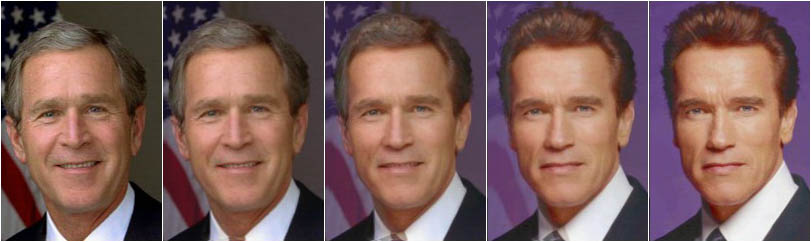
\includegraphics[scale=0.5, trim = 0 1.1cm 0 0, clip]{Pictures/Striscia_morphing.jpg}
\caption{Processo di morphing con alcuni risultati intermedi.}\label{fig:figura}
\end{figure}

\noindent
Durante la dissolvenza dall'immagine iniziale a quella finale, le immagini vengono deformate facendo in modo che ciascun punto chiave si muova lungo il percorso che porta dalla sua posizione nell'immagine di partenza alla posizione del corrispondente punto nell'immagine di arrivo. 
